\chapter{Range-Based Methods for High-Frequency Data In Two Dimensions} \label{chapter:3}

\section{Motivation}
Just as using the range of an asset, as opposed to only opening and closing values, improves the estimation of drift and volatility, we expect that using OCHL data for two assets can improve estimates for drift and volatility, as well as the estimate of their correlation. Accurate estimation of correlation across assets plays a key role in portfolio theory, as it allows for portfolio diversification to reduce risk. 

\section{Problem Formulation}
In the two-dimensional case, we simply extend the geometric Brownian motion model used in Chapter 2 to two dimensions:

\begin{eqnarray}
	dY_{1,s} = \mu_1 ds + \sigma_1 dW_{1,s}, \\ \label{eq:SDE-1}
	dY_{2,s} = \mu_2 ds + \sigma_2 dW_{2,s}. \label{eq:SDE-2}
\end{eqnarray}
Here we introduce correlation $\rho$ in the log prices of the two assets:
\[ Cov(W_1, W_2) = \rho. \]

Again using the Fokker-Planck Equation, we can take the system of SDEs in (\ref{eq:SDE-1}) - (\ref{eq:SDE-2}) and express the probability density of the asset price $q(y_1, y_2,s)$ as the PDE
\begin{eqnarray}
	\frac{\partial}{\partial s} q(y,s) &=& -\mu_1 \frac{\partial}{\partial y_1}q(y_1, y_2,s) -\mu_1 \frac{\partial}{\partial y_2}q(y_1, y_2,s) \nonumber \\
		&&  + \frac{1}{2}\sigma_1^2 \frac{\partial^2}{\partial y_1^2} q(y_1, y_2,s) + \frac{1}{2} \sigma_2^2 \frac{\partial^2}{\partial^2 y_2}q(y_1,y_2,s) + \rho \sigma_1 \sigma_2 \frac{\partial^2}{\partial y_1 \partial y_2} q(y_1, y_2, s) \label{eq:ch3-IV-1} \\
	q(y_1, y_2, t-1) &=& \delta(y_1-y_{1,t-1})\delta(y_2-y_{2,t-1}), \label{eq:ch3-IV-2}
\end{eqnarray}
where $y_{1,t-1}$ and $y_{2,t-1}$ are the prices at the beginning of the interval, and $\delta$ is the Dirac delta function. As in Chapter 2, we introduce the maximum and minimum observed prices of each asset, which establish the boundary conditions for the two-dimensional IC/BV problem

\begin{eqnarray}
	\frac{\partial}{\partial s} q(y,s) &=& -\mu_1 \frac{\partial}{\partial y_1}q(y_1, y_2,s) -\mu_1 \frac{\partial}{\partial y_2}q(y_1, y_2,s) \nonumber \\
		&&  + \frac{1}{2}\sigma_1^2 \frac{\partial^2}{\partial y_1^2} q(y_1, y_2,s) + \frac{1}{2} \sigma_2^2 \frac{\partial^2}{\partial^2 y_2}q(y_1,y_2,s) + \rho \sigma_1 \sigma_2 \frac{\partial^2}{\partial y_1 \partial y_2} q(y_1, y_2, s) \label{eq:ch3-IC-BV-1} \\
	q(y_1, y_2, t-1) &=& \delta(y_1-y_{1,t-1})\delta(y_2-y_{2,t-1}), \label{eq:ch3-IC-BV-2} \\
	q(y_1, y_2, s) &=& 0 \quad \mbox{for} \quad y_1 = a_{1,t}, b_{1,t} \,\, \mbox{ or } \,\, y_2 = a_{2,t}, b_{2,t}. \label{eq:ch3-IC-BV-3}
\end{eqnarray}

We use the same treatment as in Chapter 2 to transform the advection-diffusion problem in equations (\ref{eq:ch3-IC-BV-1}) - (\ref{eq:ch3-IC-BV-3}) into a purely diffusion problem. Letting $\mathbf{a} = (a_1, a_2)^T$ and $\mathbf{y} = (y_1, y_2)^T$, we once again introduce the form 
%
\[ q(\mathbf{y}, s) = \exp(\mathbf{a}^T\mathbf{y} + bs)p(\mathbf{y}, s). \]
%
Substituting the expression into the left and right-hand sides of (\ref{eq:ch3-IC-BV-1}) and equating gives us an expression for $\mathbf{a}$ and $b$ which eliminate the zeroeth and first order derivatives of $p$:

\[ b = \mu_1 a_1 + \mu_2 a_2 - \frac{1}{2}\sigma^2_1 a_1^2 - \frac{1}{2}\sigma^2_2 a_2^2 + \rho\sigma_1 \sigma_2 a_1 a_2, \]

\[ \left( \begin{array}{cc}
		\sigma_1^2 & \rho\sigma_1 \sigma_2 \\
		\rho\sigma_1 \sigma_2 & \sigma^2_2 
 \end{array} \right) \left( \begin{array}{c}
					a_1 \\ a_2 \end{array} \right) = \left( \begin{array}{c} \mu_1 \\ \mu_2 \end{array} \right). \]
Under these conditions, the advection-diffusion problem is once again reduced to a pure diffusion problem on a bounded domain:
\begin{eqnarray}
	\frac{\partial p(\mathbf{y},s)}{\partial s} &=& \frac{1}{2}\sigma_1^2 \frac{\partial^2}{\partial y_1^2} p(\mathbf{y},s) + \frac{1}{2} \sigma_2^2 \frac{\partial^2}{\partial^2 y_2}p(\mathbf{y},s) + \rho \sigma_1 \sigma_2 \frac{\partial^2}{\partial y_1 \partial y_2} p(\mathbf{y}, s), \label{eq:ch3-heat-1} \\
	p(\mathbf{y}, t-1) &=& \delta(y_1-y_{1,t-1})\delta(y_2-y_{2,t-1}), \label{eq:ch3-heat-2} \\
	p(\mathbf{y}, s) &=& 0 \quad \mbox{for} \quad y_1 = a_{1,t}, b_{1,t} \,\, \mbox{ or } \,\, y_2 = a_{2,t}, b_{2,t}. \label{eq:ch3-heat-3}
\end{eqnarray}


\section{Solution with the Method of Images}
Our first attempt to solve the two-dimensional diffusion problem was to apply the Method of Images approach in Chapter 2. The fundamental solution to the diffusion problem on an unbounded domain is the bivariate normal density with mean and covariance matrix 
\[ \boldsymbol{\mu} = (y_{1,t-1}, y_{2,t-1})^T, \qquad \boldsymbol{\Sigma} = \left( \begin{array}{cc}
															\sigma_1^2 & \rho \sigma_1 \sigma_2 \\
															\rho \sigma_1 \sigma_2 & \sigma_2^2 		
															\end{array} \right). \]
However, reflection of the fundamental solution across a certain boundary produces an image which satisfies a diffusion equation with a \textit{negated} correlation coefficient $\rho$ (Figure (\ref{fig:unmodified-reflection})), so that the differential equation satisfied by the reflected function is no longer the original PDE (note the minus sign in front of the mixed derivative term): 
\[ 
	\frac{\partial p(\mathbf{z},s)}{\partial s} = \frac{1}{2}\sigma_1^2 \frac{\partial^2}{\partial z_1^2} p(\mathbf{z},s) + \frac{1}{2} \sigma_2^2 \frac{\partial^2}{\partial^2 z_2}p(\mathbf{z},s) - \rho \sigma_1 \sigma_2 \frac{\partial^2}{\partial z_1 \partial z_2} p(\mathbf{z}, s)
\]
Hence, the summation of reflected images, although satisfying the boundary conditions in the limiting case, does not satisfy the original PDE. 

One can eliminate the correlation term $\rho$ through a change of coordinates consisting of a rotation, given by the eigenvalue decomposition of the covariance matrix, and a translation, such that the diffusion problem is reduced even further to
\[
\frac{\partial p(\boldsymbol{\zeta},s)}{\partial s} = \frac{1}{2}\tilde{\sigma}_1^2 \frac{\partial^2}{\partial \zeta_1^2} p(\boldsymbol{\zeta},s) + \frac{1}{2} \tilde{\sigma}_2^2 \frac{\partial^2}{\partial^2 \zeta_2}p(\boldsymbol{\zeta},s).
\]
However, the boundary where the solution is zero is no longer a rectangle but is instead a parallelogram. The non-orthogonality of the boundaries makes the process of reflecting the fundamental solution about the boundaries problematic. Particularly, if the angles between intersecting sides are not factors of $\pi$, repeated reflection places images within the computational domain of the problem, thereby violating the initial condition (see Figure (\ref{fig:transformed-reflection})). 

\begin{figure}[htbp]
        \centering
        \begin{subfigure}[t]{0.4\textwidth}
                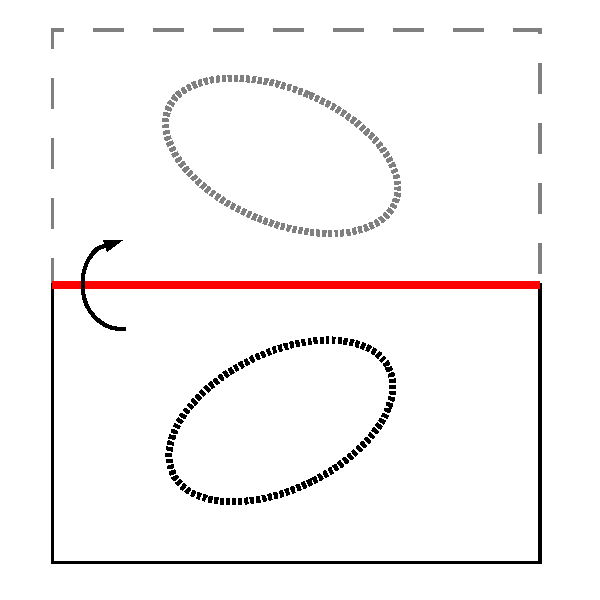
\includegraphics[width=\textwidth]{./chapter-3-two-dimensional-case/unmodified-reflection.pdf}
                \caption{When the fundamental solution (covariance ellipsoid in black) is reflected across the red boundary, the reflection has a covariance ellipsoid (gray) with a negative slope, meaning that the reflection satisfies a PDE where the correlation coefficient is negative. The sum of the fundamental solution and the reflection satisfies the boundary condition over the red line but does not satisfy the governing PDE.}
                \label{fig:unmodified-reflection}
        \end{subfigure}%
        \quad %add desired spacing between images, e. g. ~, \quad, \qquad, \hfill etc.
          %(or a blank line to force the subfigure onto a new line)
        \begin{subfigure}[t]{0.4\textwidth}
                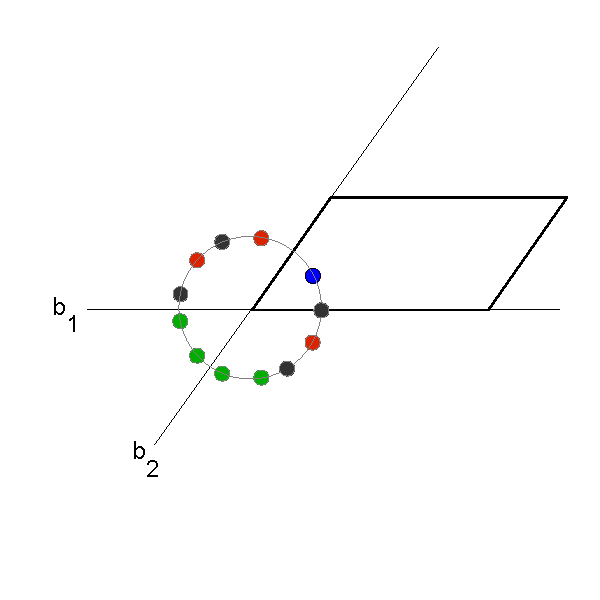
\includegraphics[width=\textwidth]{./chapter-3-two-dimensional-case/transformed-reflection.pdf}
                \caption{The fundamental solution, centered on the initial condition and denoted by the blue-inscribed red disk, is reflected alternatively around the boundaries $b_1$ and $b_2$. The displayed system of images is the results of three successive pairs of reflections around $b_1$ then $b_2$, with red corresponding to the first, green to the second, and black to the third set of reflections. We see that the system includes a fundamental solution in the computational domain in additional to the original, thereby violating the initial conditions of the problem. }
                \label{fig:transformed-reflection}
        \end{subfigure}
        
        \caption{Construction of the solution using the Method of Images}\label{fig:animals}
\end{figure}

\section{Solution by Fourier Expansion}
Similarly to the approach in Chapter 2, equation (\ref{eq:trig-expansion}), we offer a solution to the diffusion problem in terms of a trigonometric expansion of sine functions, since the basis functions must satisfy the boundary conditions:
\begin{equation}
	p(\mathbf{y}, s) = \sum_{m=1}^\infty \sum_{n=1}^\infty C_{m,n}(s) \sin\left( \frac{m \pi (y_1 - a_{1,t})}{b_{1,t} - a_{1,t}} \right) \sin\left( \frac{n \pi (y_2 - a_{2,t})}{b_{2,t} - a_{2,t}} \right)
\end{equation}	

We substitute the above form into equation (\ref{eq:ch3-heat-1}) in order to obtain expressions for $C_{m,n}(t)$:
\begin{eqnarray}
	\lefteqn{ \sum_{m=1}^\infty \sum_{n=1}^\infty \frac{dC_{m,n}(s)}{ds} \sin\left( \frac{m \pi (y_1 - a_{1,t})}{b_{1,t} - a_{1,t}} \right) \sin\left( \frac{n \pi (y_2 - a_{2,t})}{b_{2,t} - a_{2,t}} \right) =   } \nonumber \\
	&& \frac{1}{2}\sigma^2_1 \sum_{m=1}^\infty \sum_{n=1}^\infty C_{m,n}(s) \left( \frac{m\pi}{b_{1,t}-a_{1,t}} \right)^2 \sin\left( \frac{m \pi (y_1 - a_{1,t})}{b_{1,t} - a_{1,t}} \right) \sin\left( \frac{n \pi (y_2 - a_{2,t})}{b_{2,t} - a_{2,t}} \right) \nonumber \\
	&+&  \frac{1}{2}\sigma^2_2 \sum_{m=1}^\infty \sum_{n=1}^\infty C_{m,n}(s) \left( \frac{n\pi}{b_{2,t}-a_{2,t}} \right)^2 \sin\left( \frac{n \pi (y_1 - a_{1,t})}{b_{1,t} - a_{1,t}} \right) \sin\left( \frac{n \pi (y_2 - a_{2,t})}{b_{2,t} - a_{2,t}} \right) \nonumber \\
	&+& \rho \sigma_1 \sigma_2 \sum_{m=1}^\infty \sum_{n=1}^\infty C_{m,n}(s) \left( \frac{m\pi}{b_{1,t}-a_{1,t}} \right) \left( \frac{n\pi}{b_{2,t}-a_{2,t}} \right) \cos\left( \frac{m \pi (y_1 - a_{1,t})}{b_{1,t} - a_{1,t}} \right) \cos\left( \frac{n \pi (y_2 - a_{2,t})}{b_{2,t} - a_{2,t}} \right) \label{eq:expanded}
\end{eqnarray}

To deal with the cosine terms, we expand them in terms of sine functions as well, obtaining

\[
	\cos\left( \frac{m \pi (y_1 - a_{1,t})}{b_{1,t} - a_{1,t}} \right) \cos\left( \frac{n \pi (y_2 - a_{2,t})}{b_{2,t} - a_{2,t}} \right) = \sum_{k = 1}^\infty \sum_{j=1}^\infty d_{k}^{(m)} d_{j}^{(n)} \sin\left( \frac{k \pi (y_1 - a_{1,t})}{b_{1,t} - a_{1,t}} \right)\sin\left( \frac{j \pi (y_2 - a_{2,t})}{b_{2,t} - a_{2,t}} \right).
\]

Using the orthogonality of the sine and cosine series with respect to the $L^1$ norm

\[
	d^{(m)}_k = \left\{ \begin{array}{cr} 0 & \mbox{ if } k-m = \mbox{ even} \\
			\frac{4k}{\pi(k^2 - m^2)} & \mbox{ if } k-m = \mbox{ odd.} \end{array} \right.
\]
Focusing on the last line with the cosine terms
\begin{eqnarray}
	\lefteqn{ \rho \sigma_1 \sigma_2 \sum_{m=1}^\infty \sum_{n=1}^\infty C_{m,n}(s) \left( \frac{m\pi}{b_{1,t}-a_{1,t}} \right) \left( \frac{n\pi}{b_{2,t}-a_{2,t}} \right) \cos\left( \frac{m \pi (y_1 - a_{1,t})}{b_{1,t} - a_{1,t}} \right) \cos\left( \frac{n \pi (y_2 - a_{2,t})}{b_{2,t} - a_{2,t}} \right) } \label{eq:ch3-mixed-term} \\
%	&=& \rho \sigma_1 \sigma_2 \sum_{m=1}^\infty \sum_{n=1}^\infty C_{m,n}(t) \left( \frac{m\pi}{b_{1,t}-a_{1,t}} \right) \left( \frac{n\pi}{b_{2,t}-a_{2,t}} \right) \sum_{k = 1}^\infty \sum_{j=1}^\infty d_{k}^{(m)} d_{j}^{(n)} \sin\left( \frac{k \pi (y_1 - a_{1,t})}{b_{1,t} - a_{1,t}} \right)\sin\left( \frac{j \pi (y_2 - a_{2,t})}{b_{2,t} - a_{2,t}} \right) \nonumber \\
	&=& \rho \sigma_1 \sigma_2 \sum_{m=1}^\infty \sum_{n=1}^\infty \sum_{k = 1}^\infty \sum_{j=1}^\infty C_{m,n}(s) \left( \frac{m\pi}{b_{1,t}-a_{1,t}} \right) \left( \frac{n\pi}{b_{2,t}-a_{2,t}} \right) d_{k}^{(m)} d_{j}^{(n)} \sin\left( \frac{k \pi (y_1 - a_{1,t})}{b_{1,t} - a_{1,t}} \right)\sin\left( \frac{j \pi (y_2 - a_{2,t})}{b_{2,t} - a_{2,t}} \right) \nonumber
\end{eqnarray}

We want the above sine terms to be indexed by $m$ and $n$ so that the entire expression may be in the same form as the other two terms in the right-hand side of (\ref{eq:expanded}). This allows us to develop a system of ordinary differential equations for $C_{m,t}(t)$, whose solutions give $p(\mathbf{y},t)$. By Fubini's Theorem, we can exchange the order of summation in (\ref{eq:ch3-mixed-term}), relabel indexes, and group terms, obtaining 
\begin{eqnarray}
	\lefteqn{ \rho \sigma_1 \sigma_2 \sum_{m=1}^\infty \sum_{n=1}^\infty \sum_{k = 1}^\infty \sum_{j=1}^\infty C_{m,n}(s) \left( \frac{m\pi}{b_{1,t}-a_{1,t}} \right) \left( \frac{n\pi}{b_{2,t}-a_{2,t}} \right) d_{k}^{(m)} d_{j}^{(n)} \sin\left( \frac{k \pi (y_1 - a_{1,t})}{b_{1,t} - a_{1,t}} \right)\sin\left( \frac{j \pi (y_2 - a_{2,t})}{b_{2,t} - a_{2,t}} \right) } \label{eq:expanded-2} \\
	&=& \rho \sigma_1 \sigma_2 \sum_{m=1}^\infty \sum_{n=1} \left[ \sum_{k = 1}^\infty \sum_{j=1}^\infty C_{k,j}(s) \left( \frac{k\pi}{b_{1,t}-a_{1,t}} \right) \left( \frac{j\pi}{b_{2,t}-a_{2,t}} \right) d_{m}^{(k)} d_{n}^{(j)} \right] \sin\left( \frac{m \pi (y_1 - a_{1,t})}{b_{1,t} - a_{1,t}} \right)\sin\left( \frac{n \pi (y_2 - a_{2,t})}{b_{2,t} - a_{2,t}} \right) \nonumber
\end{eqnarray}
%
%To do so, we first note that 
%\begin{eqnarray*} 
%\lefteqn{ \left( \frac{m\pi}{b_{1,t}-a_{1,t}} \right) \left( \frac{n\pi}{b_{2,t}-a_{2,t}} \right) d_k^{(m)} d_j^{(n)} = \left( \frac{m\pi}{b_{1,t}-a_{1,t}} \right) \left( \frac{n\pi}{b_{2,t}-a_{2,t}} \right) \frac{4k}{\pi(k^2 - m^2)} \frac{4j}{\pi(j^2 - n^2)} } \\
%	&=& \left( \frac{k\pi}{b_{1,t}-a_{1,t}} \right) \left( \frac{j\pi}{b_{2,t}-a_{2,t}} \right) \frac{4m}{\pi(m^2 - k^2)} \frac{4n}{\pi(n^2 - j^2)} = \left( \frac{k\pi}{b_{1,t}-a_{1,t}} \right) \left( \frac{j\pi}{b_{2,t}-a_{2,t}} \right) d_{m}^{(k)} d_{n}^{(j)}.
%\end{eqnarray*}
Now plugging (\ref{eq:expanded-2}) into (\ref{eq:expanded}) we can obtain the following matrix representation for the system of ODEs for the coefficients $C_{m,n}(s)$. Truncating the expansion to a finite $M$ and $N$ terms over the indexes $m$ and $n$ respectively, the system has the form
\begin{equation}
	\frac{d}{ds} \left( \begin{array}{c} 
			C_{1,1}(s) \\
			C_{1,2}(s) \\
				\vdots \\
			C_{1,N}(s) \\
			C_{2,1}(s) \\
				\vdots \\
			C_{2,N}(s) \\
				\vdots \\
			C_{M,N}(s)
		\end{array} \right) = \frac{1}{2}\sigma^2_1 \mathbf{A}_1 + \frac{1}{2}\sigma^2_2 \mathbf{A}_2 + \rho\sigma_1 \sigma_2 \mathbf{B} \left( \begin{array}{c} 
			C_{1,1}(s) \\
			C_{1,2}(s) \\
				\vdots \\
			C_{1,N}(s) \\
			C_{2,1}(s) \\
				\vdots \\
			C_{2,N}(s) \\
				\vdots \\
			C_{M,N}(s)
		\end{array} \right) \label{eq:matrix-representation}
\end{equation}
where $\mathbf{A}_1, \mathbf{A}_2,$ and $\mathbf{B}$ are matrices of size $M \times N$. We can map from the tuple $(m,n)$ to $r$, the index of the column vector containing the $C_{m,n}(t)$ terms, via the transformation $r = (m-1)N + n$. The inverse of the transformation is $m = \xi(r) = \mbox{ceil}(r/N)$ and $n = \nu(r) = \mbox{mod}(r-1,N) + 1$. Both $\mathbf{A}_1$ and $\mathbf{A}_2$ are diagonal matrices with entries 
\[ \left[ \mathbf{A}_1 \right]_{r,r} = \left( \frac{\xi(r) \pi}{b_{1,t} - a_{1,t} } \right)^2, \]
\[ \left[ \mathbf{A}_1 \right]_{r,r} = \left( \frac{\nu(r) \pi}{b_{2,t} - a_{2,t} } \right)^2. \]
The matrix $\mathbf{B}$ is not diagonal and has entries 
\[ \left[ \mathbf{B} \right]_{r,s} = \left( \frac{\xi(s) \pi}{b_{1,t} - a_{1,t}} \right) \left( \frac{\nu(s) \pi}{b_{2,t} - a_{2,t}} \right) d_{\xi(r)}^{(\xi(s))} d_{\nu(r)}^{(\nu(s))}.  \]
Letting 
\begin{equation}
	\mathbf{A} = \frac{1}{2}\sigma^2_1 \mathbf{A}_1 + \frac{1}{2}\sigma^2_2 \mathbf{A}_2 + \rho\sigma_1 \sigma_2 \mathbf{B} \label{eq:ch3-system-matrix}
\end{equation}

\[ \mathbf{C}(s) = (C_{1,1}(s), C_{1,2}(s), \ldots, C_{1,N}(s), \ldots, C_{M,N}(s) )^T \]
the system can be written simply as 
\[ \frac{d}{ds} \mathbf{C}(s) = \mathbf{A} \mathbf{C}(s). \]
Due to the fact that $\mathbf{B}$ is a symmetric matrix, $\mathbf{A}$ is invertible, so that its eigenvalue decomposition exists. Denoting the eigenvector and eigenvalue matrices as $\mathbf{V}^T$ and $\boldsymbol{\Lambda}$, respectively, the solution to the system is given by 
\[ \mathbf{C}(t) = \exp(\mathbf{A}t)\mathbf{C}(0) = \left( \mathbf{V} \exp(\boldsymbol{\Lambda}t) \mathbf{V}^T \right) \mathbf{C}(0). \]
The vector $\mathbf{C}(0)$ is found by expanding the initial condition to the diffusion problem with sine basis functions. 

It should be noted here that if $\rho = 0$, the third term in the right-hand side of equation (\ref{eq:matrix-representation}) drops. Hence, the problem is reduced to two independent single-dimensional problems, whose solutions were found in Chapter 2. Because $\mathbf{A}_1$ and $\mathbf{A}_2$ are diagonal, under this scenario the number of terms $N$ and $M$ needed to obtain good accuracy is relatively small. However, for nonzero $\rho$, $\mathbf{B}$ is non-diagonal and dense.
%, and what is worse: dense, means that the accuracy of the expansion significantly drops for the same size of $N$ and $M$. This strongly suggests that a better basis representation is needed for computationally efficient solution to this problem. 

\section{Finding the Likelihood for the Closing Prices}
Using the shorthand 
\[ s_{m,n} = \sin\left( \frac{m \pi (y_1 - a_{1,t})}{b_{1,t} - a_{1,t}} \right) \sin\left( \frac{n \pi (y_2 - a_{2,t})}{b_{2,t} - a_{2,t}} \right), \]
the vector
\[ \mathbf{s} = ( s_{1,1}, s_{1,2}, \ldots, s_{1,N}, s_{2,1}, \ldots s_{M,N} )^T \]
contains the bases for the trigonometric expansion in the problem. The solution to the advection-diffusions problem is therefore 
\[ 
	q(\mathbf{y}, s) = \exp(\mathbf{a}^T \mathbf{y} + bs)( \exp(\mathbf{A} s) \mathbf{C}(0))^T \mathbf{s}. 
\]
To obtain the likelihood for the OCHL data in this model, we need to once again differentiate $q$ with respect to the boundary values. Since there are four boundaries, this will be a fourth-order derivative.
%
\[ 
P(m_{1,t} = a_{1,t}, m_{2,t} = a_{2,t}, M_{1,t} = b_{1,t}, M_{2,t} = b_{2,t}, Y_{1,t} = y_1, Y_{2,t} = y_2 |Y_{1,t-1}=y_{1,t-1}, Y_{2,t-1}=y_{2,t-1} )  =  
\]
%
\begin{equation} 
\frac{\partial^4 q(\mathbf{y}, t)}{\partial a_{1,t} \partial a_{2,t} \partial b_{1,t} \partial b_{2,t} } \label{eq:likelihood-bivariate}
\end{equation}
%
The simplest approach to computing the above derivative is by using a numerical differentiation scheme. Hence, the likelihood in equation (\ref{eq:likelihood-bivariate}) is initially computed using a second-order, four-point sentcil numerical differentiation scheme in line with that used in Chapter \ref{chapter:2}. A major limitation of numerical differentiation of higher orders is the finite precision of number representation systems in digital computers where the attributed round-off error is of order $10^{-16}$. When $\mathcal{O}(\Delta x^4) < 10^{-16}$, the effect of the round-off error contributes $\mathcal{O}(1)$ to the error in the numerical derivative. The limitations of using a purely numerical scheme to compute the likelihood is evident in our simulations. 

An alternative approach is to compute the derivatives analytically. The high-order derivatives of the vectors $\mathbf{C}(0)$ and $\mathbf{s}$ can be readily found. However, this is not the case for the matrix $e^{\mathbf{A}s}$. The application of a function to a matrix is defined in terms of its eigenvalue decomposition 
\[ \exp(\mathbf{A}s) = \mathbf{V} \exp(\boldsymbol{\Lambda}t) \mathbf{V}^T. \]
Since the eigenvalues and eigenvectors of the system matrix are dependent upon the boundary values, and we have no closed form expression for the eigenvalues and eigenvectors, we must define the analytic derivatives of $\exp(\mathbf{A}s)$ in terms of $\mathbf{V}$ and $\boldsymbol{\Lambda}$. \cite{wilcox1967exponential} provides the analytic expressions for second-order derivatives of functions of matrices. In general, if a function $f$ is analytic and a matrix $\mathbf{H}$ is positive-definite, 
\[ 
	\mathbf{v}_i^T \frac{\partial^2 f(\mathbf{H})}{\partial a_t \partial b_t} \mathbf{v}_j = \mathbf{v}_i^T ( \mathbf{A}_{a_t b_t} + \mathbf{A}_{b_t a_t} + \mathbf{B}_{a_t b_t} ) \mathbf{v}_j,
\]
where
% 
\begin{equation} 
	\mathbf{v}_i^T \mathbf{A}_{a_t b_t} \mathbf{v}_j = \sum_{l} \mathbf{v}_i^T \frac{\partial \mathbf{H}}{\partial a_t}  \mathbf{v}_l \mathbf{v}_l^T \frac{\partial \mathbf{H}}{\partial b_t} \mathbf{v}_j  S_{ilj} \label{eq:Aab}
\end{equation}
%
and
%
\begin{equation} 
	\mathbf{v}_i^T \mathbf{B}_{a_t b_t} \mathbf{v}_j = \mathbf{v}_i^T \frac{\partial^2 \mathbf{H}}{\partial a_t \partial b_t}  \mathbf{v}_j T_{ij}. \label{eq:Bab}
\end{equation}
%
In equations (\ref{eq:Aab}) and (\ref{eq:Bab}), $S_{ilj}$ and $T_{ij}$ are defined by 
%
\begin{eqnarray*}
	S_{ilj} &=& \frac{1}{2} \Delta_{il}\Delta_{lj} f''( \lambda_{i} ) + U_{ilj} + U_{jil} + U_{lji}, \\
	T_{ij} &=& \Delta_{ij} f'(\lambda_i) + \rho_{ij} \frac{ f(\lambda_i) - f(\lambda_j) }{\lambda_{i} - \lambda_{j} },
\end{eqnarray*}
%
where 
%
\begin{equation}
	\Delta_{ij} \equiv 1 - \rho_{ij} \equiv \left\{ \begin{array}{lr} 
											1, & \lambda_i = \lambda_j, \\
											0, & \lambda_i \neq \lambda_j,				
										\end{array}		
									\right.
\end{equation}
%
\begin{equation}
	U_{ilj} \equiv \frac{\rho_{il} \rho_{lj} \rho_{ji} f(\lambda_i) }{(\lambda_i - \lambda_l)(\lambda_{i} - \lambda_{j})} + \Delta_{il}\rho_{lj} \left[ \frac{ f(\lambda_j) - f(\lambda_i) }{(\lambda_j - \lambda_i)^2} - \frac{ f'(\lambda_i) }{\lambda_j - \lambda_i} \right].
\end{equation}
The same technique as in \cite{wilcox1967exponential} can be used to derive analytic expressions for higher-order derivatives. However, these expressions proved to be too cumbersome to be used effectively.

With the above expressions, the derivative in equation (\ref{eq:likelihood-bivariate}) is computed by first finding second-order derivatives analytically, with respect to $a_{1,t}$ and $b_{1,t}$, while the remaining differentiation is completed numerically using the same scheme as in Chapter 2, leading to an error of $\mathcal{O}(\Delta x^2)$. Particularly, we first compute using the analytic expressions above
\[ 
	\frac{\partial^2 q(\mathbf{y}, t)}{\partial a_{1,t} \partial b_{1,t}} \equiv g(a_{2,t}, b_{2,t}),
\]
after which the final derivative is found numerically
\[ 
	\frac{\partial^4 q(\mathbf{y}, t)}{\partial a_{1,t} \partial b_{1,t} \partial a_{2,t} \partial b_{2,t}} = \frac{ g(a_{2,t}+\Delta x, b_{2,t}+\Delta x) - g(a_{2,t}-\Delta x, b_{2,t}+\Delta x) - g(a_{2,t}+\Delta x, b_{2,t}-\Delta x) + g(a_{2,t}-\Delta x, b_{2,t}-\Delta x) }{4 \Delta x^2}.
\]

To understand the accuracy of the purely numerical and mixed approaches to computing the likelihood, we considered are five simulations over a nominal period of length 1 based on a forward-Euler discretization scheme of the governing stochastic differential equations:
\begin{eqnarray*} 
	Y_{1, k+1} &=& Y_{1,k} + \mu_1 \Delta t^* + \sigma_1 \Delta t^* \epsilon_{1,k}, \\
	Y_{2, k+1} &=& Y_{2,k} + \mu_2 \Delta t^* + \sigma_2 \Delta t^* \epsilon_{1,k}.
\end{eqnarray*}
with $\Delta t^* = 1/23,400$, $\epsilon_{1,k}, \epsilon_{2,k} \sim N(0,1)$, and the correlation between the two innovations is $\rho$.  This is equivalent to sampling the returns once every second over the length of a trading day. Further, 
\[ \mu_{1,2} = 0, \qquad \sigma_{1,2} = 1, \qquad \rho = (0,0.3,0.5) \]
As in Chapter 2, for each simulation there is a recorded min, max, and closing value, while all open log prices are set to 0. The likelihood is evaluated at the closing return using the observed minima and maxima, as well as the true $\mu, \sigma$ and $\rho$ used to generate the data. When performing numerical differentiation, the numerical discretization method is used with a discretization step
\[ 
	\Delta x = \min\left\{ \frac{1}{2^k} \frac{1}{100} (b_{1,t} - a_{1,t}), \frac{1}{2^k} \frac{1}{100} (b_{2,t} - a_{2,t}) \right\}
\]
Values of the likelihoods are considered across ranges of the number of expansion terms $N = M$ and $k$. Numerical and mixed differentiation results are compared. The results are shown in Tables (\ref{table:ch3-m8-rho-5}) - (\ref{table:ch3-m8-mixed-rho-0}). 

Table (\ref{table:ch3-m8-rho-0.3}), where likelihoods are found purely numerically, contains $-\infty$ entries, which is an indication that the numerical differentiation failed. This is corroborated by Table (\ref{table:ch3-m8-mixed-rho-0.3}), where likelihoods are computed using the mixed approach for the same data, and the table contains no such entries. The same derivatives are computed in Tables (\ref{table:ch3-m6-mixed-rho-0.3}) and (\ref{table:ch3-m6-rho-0.3}), where the $\Delta x$ factor is now greater since $k=6$ is used instead of $k=8$. We see no $-\infty$ entries, and further the values for mixed versus purely numerical differentiation are closer than those obtained with a smaller differentiation step, suggesting that a factor of $k=6$ strikes the balance between numerical accuracy without running into issues related to round-off error. Further, although small, the discrepancies between derivatives obtained through the mixed method and those obtained with a purely numerical scheme suggest the utility of finding and using the expressions for the analytic fourth-order derivatives of $q(\mathbf{y}, t)$. 

Finally, for $\rho = 0$, (Tables (\ref{table:ch3-m8-rho-0}) and (\ref{table:ch3-m8-mixed-rho-0})), we see a clear convergence of likelihood values across $N=M$. This is expected, as in this case we are solving two independent univariate problems that inherit the efficiency of the method in Chapter \ref{chapter:2}. For moderate $\rho = 0.3$ (Tables (\ref{table:ch3-m8-rho-0.3}) and (\ref{table:ch3-m8-mixed-rho-0.3})) and higher $\rho = 0.5$ (Tables (\ref{table:ch3-m8-rho-5}) and (\ref{table:ch3-m8-mixed-rho-5})), we do not see a clear convergence of the likelihood values as $N$ increases, meaning that the expansions used in the computations need to be greater. However, the system matrix size for $N = 64$ is already prohibitively large being $4096 \times 4096$ in terms  of eigenvalue decomposition schemes for dense matrices. This in turn suggests the need for a more efficient basis expansion of the solution to the diffusion problem. 

\begin{table}[h]
	\centering
	\csvautotabular{./chapter-3-two-dimensional-case/table-m-8-rho-5.csv}
	\caption{Likelihood values for simulations obtained via numerical differentiation with $k=8$ ( $\Delta x = 1/(100 \cdot 2^8) \cdot (b_t-a_t)$) and $\rho = 0.5$ }
	\label{table:ch3-m8-rho-5}
\end{table}

\begin{table}[h]
	\centering
	\csvautotabular{./chapter-3-two-dimensional-case/mixed-table-m-8-rho-5.csv}
	\caption{Likelihood values for simulations obtained via mixed differentiation with $k=8$ ( $\Delta x = 1/(100 \cdot 2^8) \cdot (b_t-a_t)$) and $\rho = 0.5$ }
	\label{table:ch3-m8-mixed-rho-5}
\end{table}

\begin{table}[h]
	\centering
	\csvautotabular{./chapter-3-two-dimensional-case/table-m-8-rho-3.csv}
	\caption{Likelihood values for simulations obtained via numerical differentiation with $k=8$ ( $\Delta x = 1/(100 \cdot 2^8) \cdot (b_t-a_t)$) and $\rho = 0.3$ }
	\label{table:ch3-m8-rho-0.3}
\end{table}

\begin{table}
	\centering
	\csvautotabular{./chapter-3-two-dimensional-case/mixed-table-m-8-rho-3.csv}
	\caption{Likelihood values for simulations obtained via mixed differentiation with $k=8$ ( $\Delta x = 1/(100 \cdot 2^8) \cdot (b_t-a_t)$) and $\rho = 0.3$. }
	\label{table:ch3-m8-mixed-rho-0.3}
\end{table}

\begin{table}
	\centering
	\csvautotabular{./chapter-3-two-dimensional-case/table-m-8-rho-0.csv}
	\caption{Likelihood values for simulations obtained via numerical differentiation with $k=8$ ( $\Delta x = 1/(100 \cdot 2^8) \cdot (b_t-a_t)$) and $\rho = 0$ }
	\label{table:ch3-m8-rho-0}
\end{table}


\begin{table}
	\centering
	\csvautotabular{./chapter-3-two-dimensional-case/mixed-table-m-8-rho-0.csv}
	\caption{Likelihood values for simulations obtained via mixed differentiation with $k=8$ ( $\Delta x = 1/(100 \cdot 2^8) \cdot (b_t-a_t)$) and $\rho = 0$. }
	\label{table:ch3-m8-mixed-rho-0}
\end{table}


\begin{table}
	\centering
	\csvautotabular{./chapter-3-two-dimensional-case/table-m-6-rho-3.csv}
	\caption{Likelihood values for simulations obtained via numerical differentiation with $k=6$ ( $\Delta x = 1/(100 \cdot 2^6) \cdot (b_t-a_t)$) and $\rho = 0.3$ }
	\label{table:ch3-m6-rho-0.3}
\end{table}

\begin{table}
	\centering
	\csvautotabular{./chapter-3-two-dimensional-case/mixed-table-m-6-rho-3.csv}
	\caption{Likelihood values for simulations obtained via mixed differentiation with $k=6$ ( $\Delta x = 1/(100 \cdot 2^6) \cdot (b_t-a_t)$) and $\rho = 0.3$. }
	\label{table:ch3-m6-mixed-rho-0.3}
\end{table}


%\section{A More Efficient Basis Representation: Bernstein Polynomials}
%An inefficiency of the Fourier expansion for the problem is that the mixed-derivative term contains cosine functions, whose representation in terms of the sine basis functions is given by an infinite sum. Because of this, the system matrix $\mathbf{A}$ given in equation (\ref{eq:ch3-system-matrix}) is dense. Therefore, even a modest expansion in terms of $M$ and $N$ poses computational difficulties as the size of $\mathbf{A}$ is $M \times N$. 